\section{Introduction to Detection Theory}
\label{sec:SDT}

Once we have presented some of the main concepts involved in detection problems through a series of examples, we are ready to formalize the theory for the case of two or more hypotheses.

\subsection{Hypotheses-based problems}
\label{subsec:hypotheses_problems}

As we have already explained, in this course, we will only cover a particular class of detection or classification problems to which we will refer as {\em hypotheses-based problems}. The goal is to infer the correct hypothesis, which cannot be directly observed, from a set of measurements or observations.  Thus, we consider a scenario with $M$ hypotheses, and denote the random variable that identifies the hypothesis as $H$. This is depicted in Fig. \ref{fig:clas_overview}, where $H \in \{0, 1, \ldots, M-1\}$. We also assume that we have access to an observation vector $\bf x$, which can be considered as the realization of a random variable $\bf X$ lying in observation space $\cal X$. We assume also that there is a certain statistical relationship between $H$ and $\bf X$. Otherwise, i.e., if $H$ and $\bf X$ were independent, it would make no sense to use $\bf x$ to make an informed inference about the value of $H$.

    \begin{figure}
        \begin{center}
            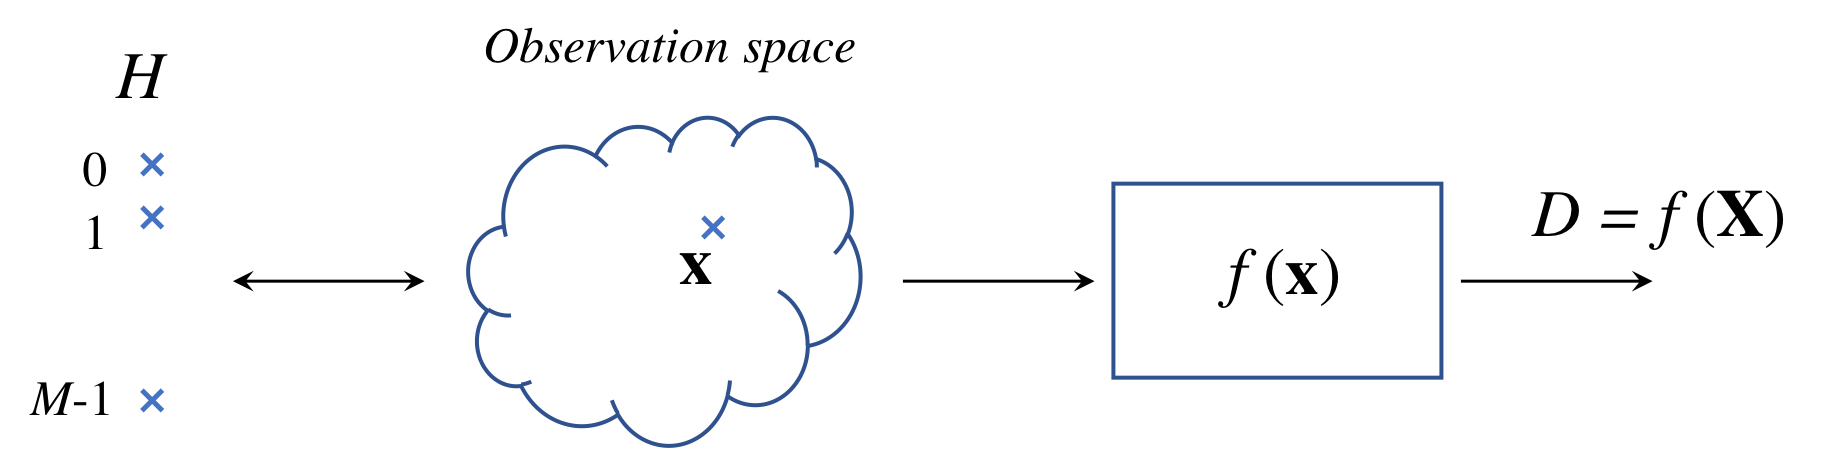
\includegraphics[width=10cm]{Figures//classification_overview.png}
        \end{center}
        \caption{Diagram block of hypothesis testing problems.\label{fig:clas_overview}}
    \end{figure}

In this context, a detector or classifier is a function of $\bf x$ that outputs a value $d$ in the range $\{0, 1, \ldots M-1\}$, i.e., a guess on the value of the hypothesis that is unknown beforehand. We should make a few considerations about the functions $f({\bf x})$ that we admit as valid detectors in this course:

\begin{itemize}
    \item We consider that $d = f({\bf x})$ is a deterministic function. This implies that if the same vector is presented several times, the function will output the same value each time. Note that, even though $f(\cdot)$ is deterministic, its output can be modeled as a random variable since the input is the random vector $\bf X$.
    \item The function is surjective, that is, every input ${\bf x}$ generates one and only one output. Hence, the function divides the observation space into $M$ non-overlapping regions, ${\cal X}_d$, $d = 0, 1, \ldots M-1$, i.e., one region per hypotheses. Moreover, the boundaries between regions are known as decision boundaries.
\end{itemize}

\begin{example}
The detector $f(x) = u(x^2 -1)$, where $u(\cdot)$ is the step function, is defined for any $x$ on the real line, and is characterized by the following decision regions:
\begin{align}{\cal X}_0 & = \left\{ x \in \Re | x^2-1 < 0\right\} = (-1,1) \nonumber\\
{\cal X}_1 & = \left\{ x \in \Re | x^2-1 \geq 0\right\} = (-\infty,-1] \cup [1,\infty) \nonumber
\end{align}
where we have assumed $u(0)=1$. In this example, the regions are connected and non-empty.
\end{example}

\begin{example}
\label{ex:decisionregions}
The decisor $f({\bf x}) = \arg\min_i y_i({\bf x})$ defined over ${\cal X} = [0,1]^2$, with
\begin{align}
y_0({\bf x}) & = \|{\bf x}\|^2 \nonumber \\
y_1({\bf x}) & = x_1 - x_0 +1 \nonumber \\
y_2({\bf x}) & = x_0 - x_1 + 1 \nonumber 
\end{align}
is characterized by the decision regions depicted in Fig. \ref{fig:decisionregions}.

    \begin{figure}
        \begin{center}
            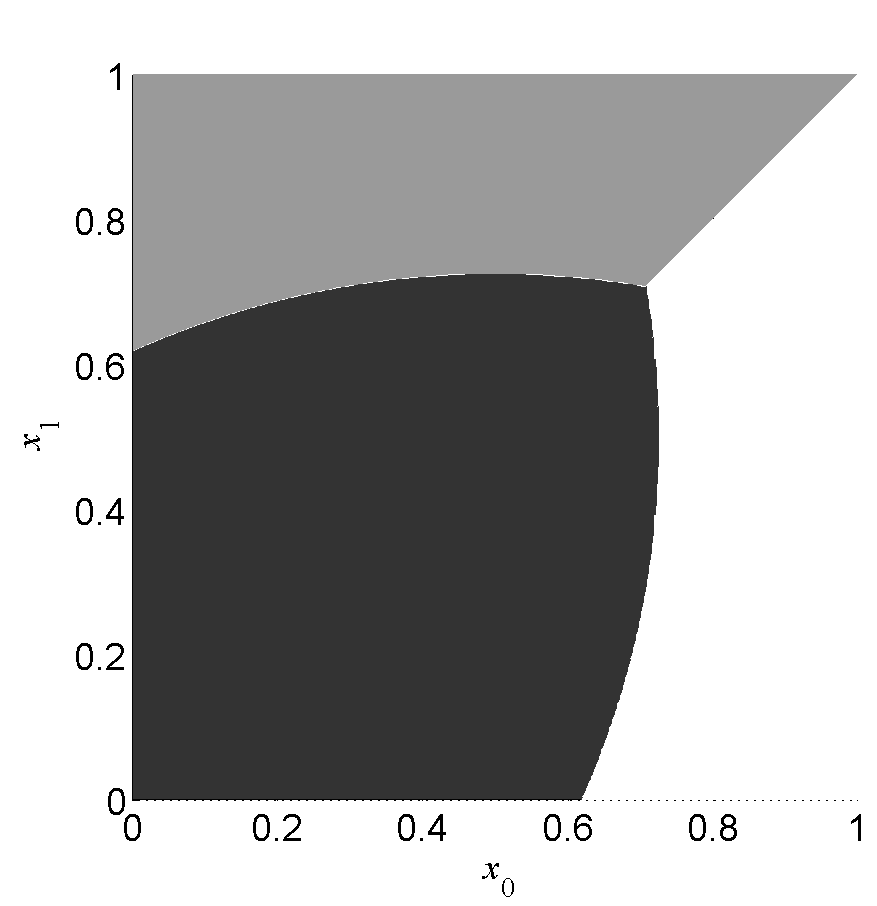
\includegraphics[width=6cm]{Figures//DecRegEx.pdf}
        \end{center}
        \caption{Decision regions for the detector given in Example \ref{ex:decisionregions}: ${\cal X}_0$ (black), ${\cal X}_1$ (grey), and ${\cal X}_2$ (white).\label{fig:decisionregions}}
    \end{figure}
    
\end{example}

\subsection{Statistical information involved in detection problems}
\label{subsec:statistical_info}

We review now the main distributions that will be employed in detection problems:
\begin{itemize}
    \item {\em A priori} probability distribution of the hypotheses: This is a discrete distribution that quantifies the probability of each hypothesis independently of the observations. If we did not have access to any observations, our design would have to rely entirely on these probabilities, as it was the case in Section \ref{subsec:example1},
    $$P_H(h), \qquad \text{ for } \quad h = 0, 1, \ldots,\;M-1.$$
    
    \item Likelihoods of the hypotheses: This represents the probability of the observations given the hypothesis. Note that, even though we refer to these distribution as the likelihoods of the hypotheses, what we actually have is a collection of distributions over the random variable $X$ (unidimensional case) or ${\bf X}$ (multidimensional case), one for each hypothesis,
    $$p_{{\bf X}|H}({\bf x}|h) \qquad \text{ for } \quad {\bf x} \in {\cal X} \text{ and } h = 0, 1, \ldots,\; M-1.$$
    where we have assumed a multidimensional case with continuous observations. Note that random variable $\bf X$ may lie in different regions depending on the hypothesis.
    
    \item {\em A posteriori} distribution of the hypotheses: This distribution provides information about the probabilities of the hypothesis, but conditioning them on each possible value of the observation vector
    $$P_{H|{\bf X}}(h|{\bf x}), \qquad \text{ for } \quad h = 0, 1, \ldots,\; M-1.$$
    Since designing a detector consists in deciding what should be the decision for each value of the observation vector, and this distribution expresses directly what are the probabilities of the hypothesis conditioned on every $\bf x$, {\em a posteriori} probabilities play a fundamental role for the statistical design of detectors. 
    
\end{itemize}

{\em A priori} and {\em a posteriori} probabilities are related by Bayes' Theorem, which states
    $$P_{H|{\bf X}}(h|{\bf x}) = \frac{p_{{\bf  X} | H}({\bf x}|h) P_H(h)}{p_{\bf X}({\bf x})}.$$
Bayes' Theorem shows how observing $\bf x$ modifies the information about the probabilities of the different hypotheses. Without them, we could only use $P_H(h)$ to make decisions. However, once the observation vector comes into play, a more accurate estimation of these probabilities can be achieved via $P_{H|{\bf X}}(h|{\bf x})$, and these probabilities can be used to obtain a more informed decision. Note also that if we know both the {\em a priori} probabilities of the hypothesis and their likelihoods, the joint distribution of $\bf X$ and $H$ can be calculated. This joint distribution is the most complete characterization of the random variables, and from it any other probability function can be calculated as well.

In the following, we consider two different kinds of problems involving $M$-ary hypothesis testing problems:
\begin{itemize}
	\item Analysis of detectors: Here, the detector is given, and the objective is to analyze its performance with respect to certain performance metrics.
	\item Detector design: The goal is to build a function $f(\bf x)$ to optimize a performance metric.
\end{itemize}

\section{Analysis of the detection performance}
\label{subsec:analysis}

The first problem that we consider is the evaluation of the performance of a given detector. In this section, we review different metrics that can be used to assess performance. In all cases, we consider first the multiple hypothesis test scenario, and afterwards we specialize it to the binary case.

\subsection{Probability of error}

The probability of error is the probability of a wrong decision, i.e., the output of the statistic is not equal to the actual hypothesis. Under a frequentist approach, this probability can be interpreted as the average number of experiments in which an incorrect decision is taken, when the number of experiments tends to infinity. However, since we are assuming that the statistical characterization of the problem is available through the different probability distributions that we just reviewed, the probability of error can be calculated in closed-form as:
\begin{align}
    P_e = P(D\neq H) & = 1 - P(D=H) \nonumber \\
    & = 1 - \sum_{h=0}^{M-1} P(D=h, H=h) \nonumber \\
    & = 1 - \sum_{h=0}^{M-1} P(D=h| H=h) P_H(h) \nonumber \\
    & = 1 - \sum_{h=0}^{M-1} P_H(h) \int_{{\cal X}_h} p_{{\bf X}|H}({\bf x}|h) d{\bf x}\nonumber
\end{align}
where we have exploited that the probability of error is one minus the probability of correct decision. This is , in most cases, more convenient since the number of combinations where $D$ and $H$ are equal is (much) smaller than the number of combinations where they differ. Moreover, the last line of the previous expression follows from
$$P(D=h| H=h) = P({\bf x}\in {\cal X}_d| H=h) = \int_{{\cal X}_h} p_{{\bf X}|H}({\bf x}|h) d{\bf x},$$
which states that, conditioned on $H=h$, the probability of $D=h$ is precisely the integral of the likelihood of that hypothesis in the region where the given detector decides in favor of hypothesis $h$, i.e., the region ${\cal X}_h$.

Finally, note that it is also possible to compute the probability of error for a particular observation vector ${\bf x}$. If ${\bf x}$ belongs to ${\cal X}_d$, the associated probability of error would be
\begin{equation}
    P(H\neq d|{\bf x}) = 1 - P( H = d|{\bf x}) = 1 - P_{H|{\bf X}}(d|{\bf x}) = \sum_{\substack{l = 0 \\ l \neq d}}^{M-1} P_{H|{\bf X}}(l|{\bf x})
    \label{eq:Pe_x}
\end{equation}
In other words, the probability of error at a particular ${\bf x} \in {\cal X}_d$ is the sum of the {\em a posteriori} probabilities of hypothesis different from $d$ conditioned on this particular observation. For instance, imagine that in a three-hypothesis testing problem for a given ${\bf x}_o$ a detector selects hypothesis $0$. Then, the probability of error for  ${\bf x}_o$ is the sum of the probabilities of hypothesis $1$ and $2$ conditioned on ${\bf X} = {\bf x}_o$, i.e., the sum of {\em a posteriori} probabilities $P_{H|{\bf X}}(1|{\bf x}_o)$ and $P_{H|{\bf X}}(2|{\bf x}_o)$.

\subsubsection{Binary case: $P_e$, $P_\text{FA}$, $P_\text{M}$ and $P_\text{D}$}
For the binary case, contrary to the multiple hypotheses test, computing the probability of error  involves as many terms as the probability of a correct decision since
\begin{align}
    P_e & = P(D=0, H=1) + P(D=1, H=0) \nonumber \\
    & = P(D=0|H=1) P_H(1) + P(D=1|H=0) P_H(0) \nonumber
\end{align}
In the expression above we find two terms that are normally referred to as the {\em probability of false alarm} (also known as probability of Type I error or significance level) and the {\em probability of missing} (or probability of Type II error):
\begin{align}
    P_\text{FA} & = P(D=1|H=0) = \int_{{\cal X}_1} p_{{\bf X}|H}({\bf x}|0) d{\bf x} \nonumber \\
    P_\text{M} & = P(D=0|H=1) = \int_{{\cal X}_0} p_{{\bf X}|H}({\bf x}|1) d{\bf x} \nonumber
\end{align}
Similarly, the probability of detection (or power) is defined as
$$P_\text{D} = P(D=1|H=1) = 1 - P_\text{M}$$
Using these definitions, the probability of error can now be expressed more compactly as
$$P_e = P_\text{M} P_H(1) + P_\text{FA} P_H(0)$$
Interestingly, for the computation of $P_\text{FA}$ and $P_\text{M}$, only likelihoods are required. However, in order to compute the overall probability of error, we also need to know the {\em a priori} probabilities of the hypothesis.

We also introduce here an important concept for the analysis of binary hypothesis tests: the receiver operating characteristic (ROC) curve. The ROC curve plots the probability of false alarm, $P_\text{FA}$, against the probability of detection, $P_\text{D}$. Figure \ref{fig:ROC} shows the ROC curves of two different detectors, Detector 1 and Detector 2. As can be seen in this figure, the performance of Detector 2 is clearly better than that of Detector 1, since for each $P_\text{FA}$, the $P_\text{D}$ of Detector 2 is equal or larger than that of Detector 1. Moreover, both detectors perform better than a random decision whose ROC curve is also shown in the figure. One final comment is in order. For almost all detectors it is not possible to increase the probability of detection without increasing the probability of false alarm.

\begin{figure}
        \begin{center}
			\includestandalone{Figures/ROC}
	\end{center}
	\caption{ROC curves for two different detectors.\label{fig:ROC}}
\end{figure}

\subsection{Average (or mean) cost}

Using the probability of error as the unique measure of the detector's performance is not a good idea, because there are many practical scenarios where not all errors are equally critical. Imagine, for instance, a detector that discriminates whether there are or not suspicious tumor masses in a medical image. Such detector is used as a pre-diagnosis system, so that patients that can have a tumor are then explored with more accurate (but also invasive) techniques. In this case, there is a clear asymmetry between both kinds of errors: The incorrect decision that tumor masses are present would result in an unnecessary biopsy and inconvenience for the patient,but the opposite error could delay the diagnosis until a time when the process is irreversible.

To assign a penalty to different kinds of errors, we can define a cost function $$c_{DH}, \qquad D,H = 0, \ldots, M-1.$$ Such function will take as many values as combinations of decisions and hypotheses, in such a way that each particular value $c_{dh}$ is the cost of deciding $D=d$ when hypothesis $H=h$ is the true one. As already pointed out, we assume deterministic costs in this course, in the sense that the cost for each particular $d$ and $h$ is fixed. However, since the cost is a function of the random variables $D$ and $H$, it is a random variable as well, and its expected value can be computed as
$$\mathbb{E}\left\{ c_{DH}\right\} = \sum_{h=0}^{M-1} \sum_{d=0}^{M-1} c_{dh} P(D=d, H=h).$$

In order to compute the expected cost in terms of the probability distributions of ${\bf X}$ and $H$, we can use the relationship between $D$ and ${\bf X}$, which yields
\begin{align}
\mathbb{E}\left\{ c_{DH}\right\} & = \sum_{h=0}^{M-1} \sum_{d=0}^{M-1} c_{dh} P({\bf x}\in {\cal X}_d, H=h) \nonumber \\
& = \sum_{h=0}^{M-1} P_H(h) \sum_{d=0}^{M-1} c_{dh} P({\bf x}\in {\cal X}_d| H=h) \nonumber \\
& = \sum_{h=0}^{M-1} P_H(h) \sum_{d=0}^{M-1} c_{dh} \int_{{\bf x}\in {\cal X}_d} p_{{\bf X}|H}({\bf x}|h) d{\bf x}.\nonumber
\end{align}
Finally, we can also compute the expected cost conditioned on a given value of ${\bf x}$. Taking into account that, for a given ${\bf x}$ and a given detector, the decision value is fixed, it is only required to take expectations with respect to such hypothesis. Consider, for instance, the computation of the mean cost for some value ${\bf x}$ belonging to ${\cal X}_d$. Thus, the expected cost is obtained as
\begin{equation}
    \mathbb{E}\left\{ c_{dH}\right|{\bf x}\} = \sum_{h=0}^{M-1} c_{dh} P_{H|X}(h|{\bf x}).
\label{eq:cost_x}
\end{equation}

\subsubsection{Binary case: Mean cost}

For the binary case, a simpler expression can be obtained in terms of $P_\text{FA}$, $P_\text{M},$ and $P_\text{D}$ as follows
\begin{align}
    \mathbb{E}\left\{ c_{DH}\right\} & = c_{00} P(D=0, H=0) + c_{01} P(D=0,H=1) \nonumber \\
    & \;\;\;\;\;\; + c_{10} P(D=1, H=0) + c_{11} P(D=1,H=1) \nonumber \\
    & = c_{00} P(D=0|H=0) P_H(0) + c_{01} P_\text{M} P_H(1) \nonumber \\
    & \;\;\;\;\;\; + c_{10} P_\text{FA}P_H(0) + c_{11} P_\text{D} P_H(1) .\nonumber
\end{align}

\section{Detector design}
\label{subsec:design}

Once we have studied different ways of analyzing the performance of a given detector, we turn our attention to the problem of designing detectors that maximize one of these performance metrics.

\subsection{Maximum likelihood and maximum \emph{a posteriori} detectors}

A first possibility would be to rely directly on the maximization of the available probability density functions:

\begin{itemize}
    \item The detector that maximizes the likelihood is known as the {\em maximum likelihood} (ML) detector:
    $$d_{ML} = \arg\max_h p_{{\bf X}|H}({\bf x}|h).$$
    \item The detector that selects the hypothesis with maximum {\em a posteriori} probability is known as the  maximum {\em a posteriori} (MAP) detector:
    $$d_{MAP} = \arg\max_h P_{H|{\bf X}}(h|{\bf x}).$$
\end{itemize}

These detectors proceed as follows. Designing a detector is equivalent to specifying a unique decision for each possible value of the observation vector ${\bf x}$. Then, the ML and MAP strategies are based on evaluating either the likelihoods or the {\em a posteriori} probabilities for each ${\bf x}$ in the observation space, and select, for each ${\bf x}$, the hypothesis that maximizes $p_{{\bf X}|H}({\bf x}|h)$ (ML) or $P_{H|{\bf X}}(h|{\bf x})$ (MAP).

Finally, there are two properties that are worth considering with respect to these detectors:
\begin{enumerate}
    \item When the {\em a priori} probabilities of the hypothesis are the same, i.e., $P_H(h) = 1/M$, the ML and MAP detectors are identical. This can be shown from the Bayes' Theorem, since in this case
    $$d_{MAP} = \arg\max_h P_{H|{\bf X}}(h|{\bf x}) = \arg\max_h \frac{p_{{\bf X}|H}({\bf x}|h) P_H(h)}{p_{\bf X}(\bf x)} = \arg\max_h p_{{\bf X}|H}({\bf x}|h) = d_{ML}$$
    
    \item The MAP detector minimizes the probability of error. Note that according to \eqref{eq:Pe_x} the probability of error for a given $\bf x$ can be expressed as
    $$P(D\neq H|{\bf x}) = 1 - P_{ H|{\bf X}}(h|{\bf x})$$
    Since the MAP detector selects for every $\bf x$ the hypothesis that maximizes $P_{H|{\bf X}}(h|{\bf x})$, it therefore minimizes the probability of error for each vector of the observation space. Thus, as the probability of error is minimized for each point of the observation space, it is also minimized overall. That is,
    $$P(D\neq H) = \int_{\mathcal{X}} P(D\neq H|{\bf x}) p_{\bf X}(\bf x) d{\bf x},$$
    and we can check that the value of the integral (the probability of error) is minimized if, for each $\bf x$, the decisions minimize $P(D\neq H|{\bf x})$, i.e., the MAP detector.
    
\end{enumerate}

\subsubsection{Binary case: ML and MAP detectors}

The expressions of the ML and MAP detectors become fairly simple for the binary case:
\begin{itemize}
    \item Maximum likelihood detector:
    $$p_{{\bf X}|H}({\bf x}|1) \dunodcero p_{{\bf X}|H}({\bf x}|0),$$
    which can be expressed as a {\em likelihood ratio test} (LRT)
    $$\displaystyle\frac{p_{{\bf X}|H}({\bf x}|1)}{p_{{\bf X}|H}({\bf x}|0)} \dunodcero 1,$$
    where we have taken into account that the likelihoods are non-negative. Sometimes, it will be more convenient to work with the {\em log-likelihood ratio test} (LLRT)
    \begin{equation}
    \label{eq:LLRT}
    \log \left[ \frac{p_{{\bf X}|H}({\bf x}|1)}{p_{{\bf X}|H}({\bf x}|0)} \right] = \log p_{{\bf X}|H}({\bf x}|1) - \log p_{{\bf X}|H}({\bf x}|0) \dunodcero 0,
    \end{equation}
    which can be done because the logarithm is a monotonically increasing function.
    \item Maximum \emph{a posteriori} detector:
    $$p_{H|{\bf X}}(1|{\bf x}) \dunodcero p_{H|{\bf X}}(0|{\bf x}),$$
    which can also be expressed as a LRT as
    $$\displaystyle\frac{p_{{\bf X}|H}({\bf x}|1)}{p_{{\bf X}|H}({\bf x}|0)} \dunodcero \displaystyle\frac{P_H(0)}{P_H(1)}.$$
\end{itemize}

As in the general case with $M$ hypothesis, the MAP detector minimizes the probability of error and the ML and MAP detectors are the same if $P_H(0)=P_H(1)=0.5$. Moreover, we can see that both detectors can be expressed as a LRT
    $$\displaystyle\frac{p_{{\bf X}|H}({\bf x}|1)}{p_{{\bf X}|H}({\bf x}|0)} \dunodcero \eta,$$
where $\eta$ is a threshold. When this threshold is $1$, the LRT is the ML detector and for $\eta = P_H(0)/P_H(1)$, the LRT becomes the MAP detector, that is, minimum $P_e$ detector. Hence, we get two different points in the ROC curve. Actually, sweeping the value of the threshold generates the complete ROC curves in Figure \ref{fig:ROC}.\footnote{This actually applies to all detectors that can be written as $\phi({\bf x}) \dunodcero \eta$. That is, comparing a function of the observations with a threshold achieves a given $(P_\text{FA},P_\text{D})$ point in the ROC curve. These detectors are known as threshold detectors.}

\subsubsection{Binary case: Neyman-Pearson detector}

The Neyman-Pearson (NP) detector is a well known detector for binary problems, which maximizes the probability of detection while it provides a bound on the probability of false alarm. Before proceeding with the derivation, let us recall the definitions of probability of false alarm and detection
\begin{align}
P_\text{FA} & = \int_{{\cal X}_1} p_{{\bf X}|H}({\bf x}|0) d{\bf x}, \nonumber \\
P_\text{D} & = \int_{{\cal X}_1} p_{{\bf X}|H}({\bf x}|1) d{\bf x}. \nonumber
\end{align}
Now, the NP detector can be derived as the solution to
\begin{equation*}
	\text{maximize } P_\text{D}, \quad \text{subject to } P_\text{FA} = \alpha,
\end{equation*}
which is an optimization problem with constraints. The solution this kind of problems is obtained from the Lagrangian, which is given by
\begin{align}
\mathcal{L}(\mathcal{X}_1,\eta) &= P_\text{D} - \eta (P_\text{FA} - \alpha) \nonumber \\
&= \int_{{\cal X}_1} p_{{\bf X}|H}({\bf x}|1) d{\bf x}  - \eta \left(\int_{{\cal X}_1} p_{{\bf X}|H}({\bf x}|0) d{\bf x} - \alpha \right) \nonumber \\
&= \int_{\mathcal{X}_1} \left( p_{{\bf X}|H}({\bf x}|1) - \eta p_{{\bf X}|H}({\bf x}|0)  \right) d  {\bf x} + \eta \alpha \nonumber
\end{align}
Note, that the optimization variable is the region where we decide $d=1$. Next, we need to maximize the Lagrangian, and therefore the $P_\text{D}$, which is achieved by maximizing the above integral. To do so, and taken into account that an integral may be seen as a sum, we need to design ${\cal X}_1$ such that the integrand is positive, i.e.
\begin{equation*}
	\mathcal{X}_1 = \{\mathbf{x} |p_{{\bf X}|H}({\bf x}|1) - \eta p_{{\bf X}|H}({\bf x}|0) \geq 0 \} \Rightarrow \frac{p_{{\bf X}|H}({\bf x}|1)}{p_{{\bf X}|H}({\bf x}|0)} \dunodcero \eta
\end{equation*}
and $\eta$ is selected to achieve the desired probability of false alarm.

\subsection{Minimum expected cost detector}

As we have already studied, sometimes it makes more sense to measure the performance of a detector in terms of the expected cost. Therefore, it is important to tackle the problem of designing a detector that is optimum with respect to the expected cost.

Remember that the expected cost of a detector deciding $d$ for an observation ${\bf x}$ is given by equation \eqref{eq:cost_x}, which we reproduce here for convenience:
\begin{equation}
    \mathbb{E}\left\{ c_{dH}\right|{\bf x}\} = \sum_{h=0}^{M-1} c_{dh} P_{H|X}(h|{\bf x}) \label{eq:mean_x_2}.
\end{equation}
Minimizing the expected cost over the whole observation space requires that decisions for each observation minimize the conditional expected cost. That is, for each ${\bf x}$ the above expression should be minimized, and the expression of the minimum mean cost detector can be stated as follows:
$$d^\star = \arg\min_{d} \sum_{h=0}^{M-1} c_{dh} P_{H|X}(h|{\bf x})$$
Hence, when designing the detector, we need to evaluate the cost of the different decisions for each observation vector, and select the decision for which the expected cost is minimized.

It is interesting to point out that when the cost function penalizes equally all kinds of errors, i.e.,
$$c_{dh} = \left\{\begin{array}{ll} 0, & \;\;\;\;d=h \\ c, & \;\;\;\;d\neq h\end{array}\right.$$
the detector with minimum expected cost becomes the MAP one. This is easily proved by replacing these costs into the expression for the minimum expected cost detector
\begin{align}
    d^\star & = \arg\min_{d} \sum_{h=0}^{M-1} c_{dh} P_{H|X}(h|{\bf x}) \nonumber \\
            & = \arg\min_{d} \ c \sum_{h\neq d} P_{H|X}(h|{\bf x}) \nonumber \\
            & = \arg\min_{d} \sum_{h\neq d} P_{H|X}(h|{\bf x}) \nonumber \\
            & = \arg\min_{d} 1 - P_{H|X}(d|{\bf x}) \nonumber \\
            & = \arg\max_{d} P_{H|X}(d|{\bf x}) \nonumber \\
            & = d_{MAP}.
\end{align}

\subsubsection{Binary case: Minimum expected cost detector}

In the binary case, we can also express the optimum detector with respect to a cost function as an LRT. Let us start by particularizing \eqref{eq:mean_x_2} for $d=0$ and $d=1$, and then follow the criterion of deciding in favor of the minimum cost, i.e.,
$$\mathbb{E}\left\{ c_{0H}\right|{\bf x}\} \dunodcero \mathbb{E}\left\{ c_{1H}\right|{\bf x}\}.$$
Now, using the definition of expectation, the criterion becomes
$$c_{00}P_{H|{\bf X}}(0|{\bf x}) + c_{01} P_{H|{\bf X}}(1|{\bf x})\dunodcero c_{10}P_{H|{\bf X}}(0|{\bf x}) + c_{11} P_{H|{\bf X}}(1|{\bf x}),$$
which after some algebra can be rewritten as
$$\displaystyle\frac{P_{H|{\bf X}}(1|{\bf x})}{P_{H|{\bf X}}(0|{\bf x})}\dunodcero \displaystyle\frac{c_{10}-c_{00}}{c_{01}-c_{11}}.$$
Finally, using Bayes' Theorem, we may rewrite the \emph{a posteriori} probabilities in terms of the likelihoods and the \emph{a priori} probabilities, which finally yields
$$\displaystyle\frac{P_{{\bf X}|H}({\bf x}|1)}{P_{{\bf X}|H}({\bf x}|0)}\dunodcero \displaystyle\frac{c_{10}-c_{00}}{c_{01}-c_{11}} \displaystyle\frac{P_H(0)}{P_H(1)},$$
and corresponds to yet another point of the ROC curve of the LRT.

\subsection{The Gaussian case}

In this section, we will derive the likelihood ratio test for Gaussian observation under several assumptions. Then, depending on the threshold, we would obtain the different detectors: NP, ML, MAP, and minimum cost.

Before proceeding, we introduce the multivariate real Gaussian probability density function (PDF), which is given by
\begin{equation}
P_{{\bf X}}({\bf x}) = \frac{1}{(2\pi)^{N/2} |{\bf V}|^{1/2}}
\exp\left(-\frac{1}{2}({\bf x}-{\bf m})^T {\bf V}^{-1}({\bf x}-{\bf m})\right)
\label{pXGauss}
\end{equation}
where ${\bf x}$ is an $N$-dimensional vector, ${\bf m}$ is the mean vector, and ${\bf V}$ is the cross-covariance matrix. Then, under hypothesis $h = 0$, the likelihood is
\begin{equation*}
P_{{\bf X}|H}({\bf x}|0) = \frac{1}{(2\pi)^{N/2} |{\bf V}_0|^{1/2}}
\exp\left(-\frac{1}{2}({\bf x}-{\bf m}_0)^T {\bf V}_0^{-1}({\bf x}-{\bf m}_0)\right),
\end{equation*}
whereas it is
\begin{equation*}
P_{{\bf X}|H}({\bf x}|1) = \frac{1}{(2\pi)^{N/2} |{\bf V}_1|^{1/2}}
\exp\left(-\frac{1}{2}({\bf x}-{\bf m}_1)^T {\bf V}_1^{-1}({\bf x}-{\bf m}_1)\right),
\end{equation*}
under hypothesis $h = 1$. For this hypothesis test, the LLRT in \eqref{eq:LLRT} becomes
\begin{multline*}
- \frac{1}{2}\log\left|{\bf V}_1 \right| 
- \frac{1}{2}({\bf x}-{\bf m}_1)^T {\bf V}_1^{-1}({\bf x}-{\bf m}_1) \\
+ \frac{1}{2}\log\left|{\bf V}_0 \right| 
+ \frac{1}{2}({\bf x}-{\bf m}_0)^T {\bf V}_0^{-1}({\bf x}-{\bf m}_0) 
\dunodcero \log(\eta) 
\end{multline*}
or, equivalently,
\begin{align}
({\bf x}-{\bf m}_0)^T {\bf V}_0^{-1}({\bf x}-{\bf m}_0) 
- ({\bf x}-{\bf m}_1)^T {\bf V}_1^{-1}({\bf x}-{\bf m}_1)
\dunodcero \mu
\label{eq:logLRTGauss}
\end{align}
where
\begin{equation*}
\mu = 2 \log(\eta) + \log\left|{\bf V}_1 \right| - \log\left|{\bf V}_0 \right|,
\end{equation*}
with $\eta$ being a threshold selected according to the performance criterion.

After a careful look at \eqref{eq:logLRTGauss}, it can be shown that the optimal detector in the Gaussian case is given by a second-order polynomial function. Hence, the decision boundaries\footnote{We obtain the decision boundaries for the equality in \eqref{eq:logLRTGauss}.} are quadratic surfaces. For instance, for 2D problems ($N = 2$), these boundaries are hyperbolas, parabolas, ellipses or straight lines.

In the following sections, we consider a few particular cases, but we conclude this section with two examples.

\begin{example}
	Figure \ref{fig:DecGauss2Dhip} shows the decision boundaries for the ML detector ($\eta = 1$ in \eqref{eq:logLRTGauss}), for a detection problem with 2D Gaussian observations with the following means and cross-covariance matrices:
	\begin{equation*}
	{\bf m}_0 =  \left(\begin{array}{l}  1 \\ 1 \end{array}\right), {\bf V}_0 = 
	\left(\begin{array}{ll} 1.2 & 0.43 \\ 0.43 & 1.75 \end{array} \right),
	\end{equation*}
	and
	\begin{equation*}
	{\bf m}_1 = \left(\begin{array}{l}  3 \\ 3 \end{array}\right), {\bf V}_1 = 
	\left(\begin{array}{ll} 2 & 0 \\ 0 & 1 \end{array} \right).
	\end{equation*}
	In this figure, the gray color gradient  represents the value of the likelihoods $P_{{\bf X}|H}({\bf x}|0)$ and $P_{{\bf X}|H}({\bf x}|1)$, where darker colors denote larger values. Moreover, the white curves are the iso-probability lines and the black curve is the decision boundary, which in this case is a hyperbola (the symmetric part is not shown in this figure).
	
	\begin{figure}[htb]
		\begin{center}
			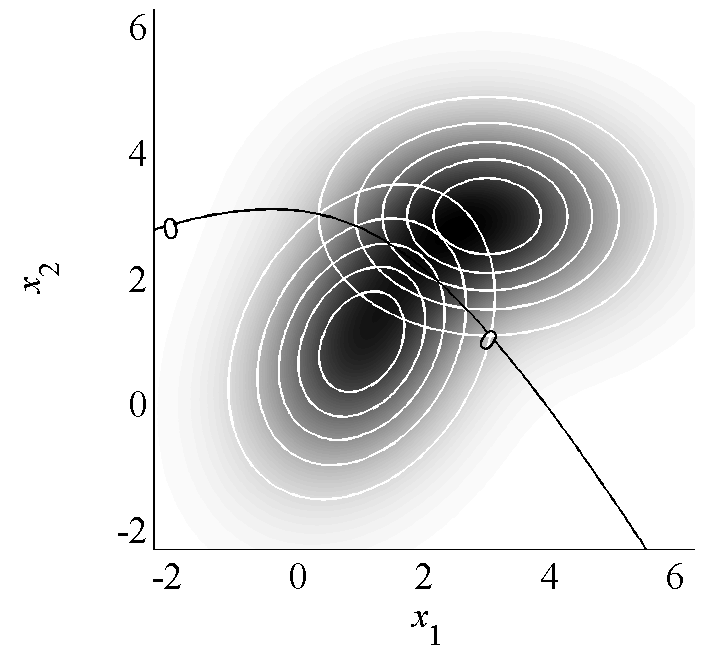
\includegraphics[width=6cm]{Figures/DecGauss2Dhip}
			\caption{Hyperbolic decision boundary of the ML detector and likelihoods for a Gaussian detection problem with 2D observations.}
			\label{fig:DecGauss2Dhip}
		\end{center}
	\end{figure}
\end{example}

\begin{example}
	Figure \ref{fig:DecGauss2Delip} shows an equivalent figure that of the previous example, but for a problem with the following means and cross-covariance matrices:
		\begin{equation*}
	{\bf m}_0 =  \left(\begin{array}{l}  0\\0  \end{array}\right), {\bf V}_0 = 
	\left(\begin{array}{ll} 0.7 & 0 \\ 0 & 0.7 \end{array} \right),
	\end{equation*}
	and
	\begin{equation*}
	{\bf m}_1 = \left(\begin{array}{l}  0.2 \\ 0.4 \end{array}\right), {\bf V}_1 = 
	\left(\begin{array}{ll} 0.5 & 0 \\ 0 & 0.2 \end{array} \right).
	\end{equation*}
	In this case, the decision boundary is an ellipse.
	\begin{figure}[htb]
		\begin{center}
			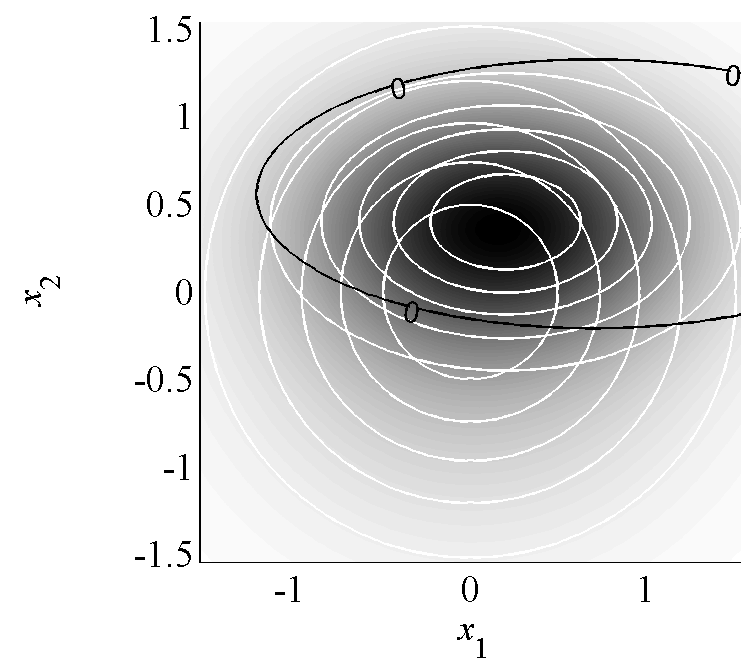
\includegraphics[width=6cm]{Figures/DecGauss2Delip.pdf}
			\caption{Elliptic decision boundary of the ML detectors and likelihoods for a Gaussian detection problem with 2D observations.}
			\label{fig:DecGauss2Delip}
		\end{center}
	\end{figure}
\end{example}

\subsubsection{Identical cross-covariance matrices}

This section considers the case of ${\bf V}_1 = {\bf V}_0 = {\bf V}$. Then, the LLRT becomes
\begin{equation*}
({\bf x}-{\bf m}_0)^T {\bf V}^{-1}({\bf x}-{\bf m}_0) 
- ({\bf x}-{\bf m}_1)^T {\bf V}^{-1}({\bf x}-{\bf m}_1)
\dunodcero \mu.
\end{equation*}
Now, expanding the quadratic forms, the above expression simplifies to
\begin{equation}
 ({\bf m}_1-{\bf m}_0)^T {\bf V}^{-1}{\bf x} \dunodcero \tilde{\mu},
 \label{eq:LLRT_Gaussian_same_Vs}
\end{equation}
where $\tilde{\mu} = \mu/2 + {\bf m}_1^T {\bf V}^{-1}{\bf m}_1/2 - {\bf m}_0^T {\bf V}^{-1}{\bf m}_0/2$. In this particular case, the LLRT in \eqref{eq:LLRT_Gaussian_same_Vs} is a linear function of the observation vector ${\bf x}$.

\begin{example}
	Figure \ref{Dec:DecGauss2Deqv} shows three decision boundaries for an example with
		\begin{equation*}
			{\bf m}_0 =  \left(\begin{array}{l}  1\\1  \end{array}\right), {\bf V}_0 = 
			\left(\begin{array}{ll} 0.44 & 0.32 \\ 0.32 & 0.81 \end{array} \right)
\end{equation*}
and
\begin{equation*}
{\bf m}_1 = \left(\begin{array}{l}  3\\3 \end{array}\right), {\bf V}_1 = 
\left(\begin{array}{ll} 0.44 & 0.32 \\ 0.32 & 0.81 \end{array} \right).
\end{equation*}
The label of each decision boundary is $\log(\eta)$. Then, $\log(\eta) = 0$ corresponds to the ML detector.
	\begin{figure}[htb]
		\begin{center}
			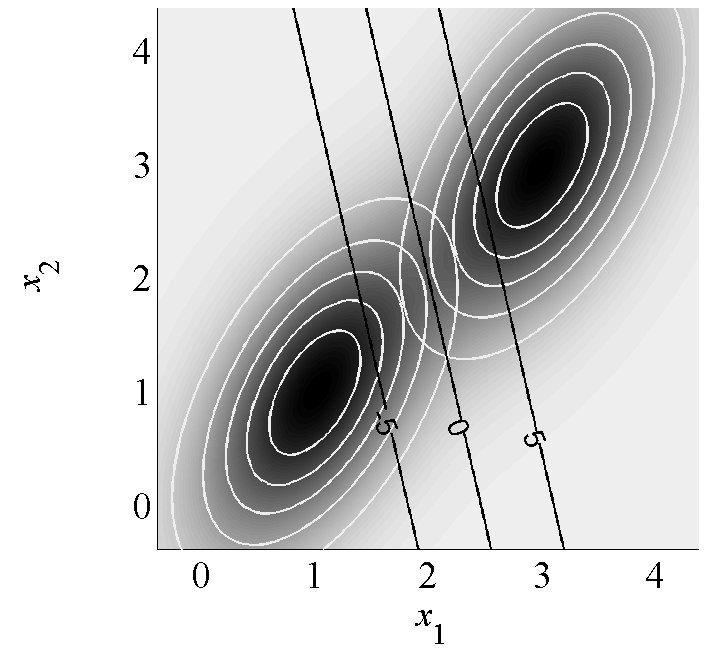
\includegraphics[width=6cm]{Figures/DecGauss2Deqv.pdf}
			\caption{Decision boundaries of the LLRT and likelihoods for a Gaussian detection problem with 2D observations and identical covariance matrices.}
			\label{Dec:DecGauss2Deqv}
		\end{center}
	\end{figure}
\end{example}

\begin{example}[Mathed filter]
	In this example, we derive one of the most well known detectors, the mathed filter (MF). The MF is the LLRT to the detection of a known signal contaminated by zero-mean Gaussian noise. Concretely, under hypothesis $h=0$, the observations are given by noise only:
	\begin{equation*}
	x[n] = w[n], \quad n = 0, \ldots, N-1,
	\end{equation*}
	and under  hypothesis $h=1$, the observations are
	\begin{equation*}
	x[n] = s[n] + w[n], \quad n = 0, \ldots, N-1,
	\end{equation*}
	where $s[n]$ is a known signal and $w[n]$ is additive white Gaussian noise with zero mean and variance $\sigma^2$, i.e., $w[n] \sim \Normal(0,\sigma^2)$. To use the LLRT already derived in this section, we must first define the vector
	\begin{equation*}
	{\bf x} = \begin{pmatrix} x[0] & x[1] & \cdots & x[N-1] \end{pmatrix}^T = {\bf s} + {\bf w},
	\end{equation*}
	with ${\bf s} = \begin{pmatrix} s[0] & s[1] & \cdots & s[N-1] \end{pmatrix}^T $ and ${\bf w} = \begin{pmatrix} w[0] & w[1] & \cdots & w[N-1] \end{pmatrix}^T$, and obtain the distributions of ${\bf x}$ under both hypothesis. Under hypothesis $h=0$, the observation vector ${\bf x}$ collects samples of a Gaussian process, which makes it also Gaussian. Hence, only the mean and cross-covariance matrices are required:
	\begin{equation*}
	{\bf m}_0 = \mathbb{E}\{{\bf x}|0\} = \mathbb{E}\{{\bf w}\} = \begin{pmatrix} \mathbb{E}\{w[0]\}  & \mathbb{E}\{w[1]\} & \cdots & \mathbb{E}\{w[N-1]\} \end{pmatrix}^T = \mathbf{0},
	\end{equation*}
    and
	\begin{align*}
		{\bf V}_0 &= \mathbb{E}\left\{({\bf x} - {\bf m}_0) ({\bf x} - {\bf m}_0)^T|0\right\} = \mathbb{E}\left\{{\bf w} {\bf w}^T\right\} \\ &= \mathbb{E}\left\{\begin{pmatrix} w[0] & w[1] & \cdots & w[N-1] \end{pmatrix}^T \begin{pmatrix} w[0] & w[1] & \cdots & w[N-1] \end{pmatrix}\right\} \\
		&= \begin{pmatrix} \mathbb{E}\left\{w^2[0]\right\}  & \mathbb{E}\left\{w[0]w[1] \right\}& \cdots & \mathbb{E}\left\{w[0]w[N-1]\right\} \\ \mathbb{E}\left\{w[1] w[0]\right\} & \mathbb{E}\left\{w^2[1]\right\} & \cdots & \mathbb{E}\left\{w[1]w[N-1]\right\} \\ \vdots & \vdots & \ddots & \vdots   \\ \mathbb{E}\left\{w[N-1] w[0]\right\} & \mathbb{E}\left\{w[N-1] w[1]\right\} & \cdots & \mathbb{E}\left\{w^2[N-1] \right\} \end{pmatrix}.
 	\end{align*}
	The cross-covariance matrix ${\bf V}_0$ can be simplified taking into account that the noise is white, i.e., $\mathbb{E}\{w[n] w[n-m]\} = \sigma^2 \delta[m]$, which yields 
	\begin{equation*}
		{\bf V}_0 = \begin{pmatrix} \sigma^2  & 0 & \cdots & 0 \\ 0 & \sigma^2 & \cdots & 0 \\ \vdots & \vdots & \ddots & \vdots   \\ 0 & 0 & \cdots & \sigma^2 \end{pmatrix} = \sigma^2 \mathbf{I}.
\end{equation*}
Similarly, under hypothesis $h=1$, the observations are Gaussian with mean
\begin{equation*}
	{\bf m}_1 = \mathbb{E}\{{\bf x}|1\} = \mathbb{E}\{{\bf s} + {\bf w}\} = \mathbb{E}\{{\bf s}\} + \mathbb{E}\{{\bf w}\} = {\bf s},
\end{equation*}
since ${\bf s}$ is deterministic, and cross-covariance matrix
	\begin{equation*}
{\bf V}_1 = \mathbb{E}\left\{({\bf x} - {\bf m}_1) ({\bf x} - {\bf m}_1)^T|1\right\} = \mathbb{E}\left\{({\bf s} + {\bf w} - {\bf s}) ({\bf s} + {\bf w} - {\bf s})^T\right\} = \mathbb{E}\left\{{\bf w} {\bf w}^T\right\} = \sigma^2 \mathbf{I}.
\end{equation*}
Hence, the detection problem is that of Gaussian observations with identical covariance matrices, for which the LLRT is
\begin{equation*}
({\bf m}_1-{\bf m}_0)^T {\bf V}^{-1}{\bf x} = \frac{1}{\sigma^2} {\bf s}^T {\bf x} \dunodcero \tilde{\mu} \Rightarrow \underbrace{\sum_{n = 0}^{N-1} s[n]x[n]}_{MF} \ \dunodcero \sigma^2 \tilde{\mu}.
\end{equation*}
Alternatively, and the motivation for the term matched filter, is because the above detector can be rewritten as a filtering of then signal $x[n]$ with the filter $h[n] = s[N-1 - n]$, followed by sampling every $N$ samples. Finally, we also would like to point out that the matched filter is a filter that maximizes the signal-to-noise ratio.

\end{example}

\subsubsection{Zero means}

We consider now that ${\bf m}_0 = {\bf m}_1 = \mathbf{0}$, which yields
\begin{equation*}
{\bf x}^T \left({\bf V}_0^{-1}-{\bf V}_1^{-1}\right){\bf x} \dunodcero \mu.
\label{eq:logLRTGauss2m0}
\end{equation*}

\begin{example}
	Figure \ref{fig:DecGauss2Deqm} shows the ML decision boundary for 2D Gaussian observations with
		\begin{equation*}
{\bf m}_0 =  \left(\begin{array}{l}  0\\0   \end{array}\right), {\bf V}_0 = 
\left(\begin{array}{ll} 0.62 & -0.22 \\ -0.22 & 0.37 \end{array} \right),
\end{equation*}
and
\begin{equation*}
{\bf m}_1 = \left(\begin{array}{l}  0\\0  \end{array}\right), {\bf V}_1 = 
\left(\begin{array}{ll} 1 & 0 \\ 0 & 2 \end{array} \right).
\end{equation*}
	The region ${\cal X}_0$ is given by the interior of the ellipse. Moreover, since the variance of the observations in every direction is larger under hypothesis $h=1$, points further away from the origin should be assigned $d=1$.
	\begin{figure}[htb]
		\begin{center}
			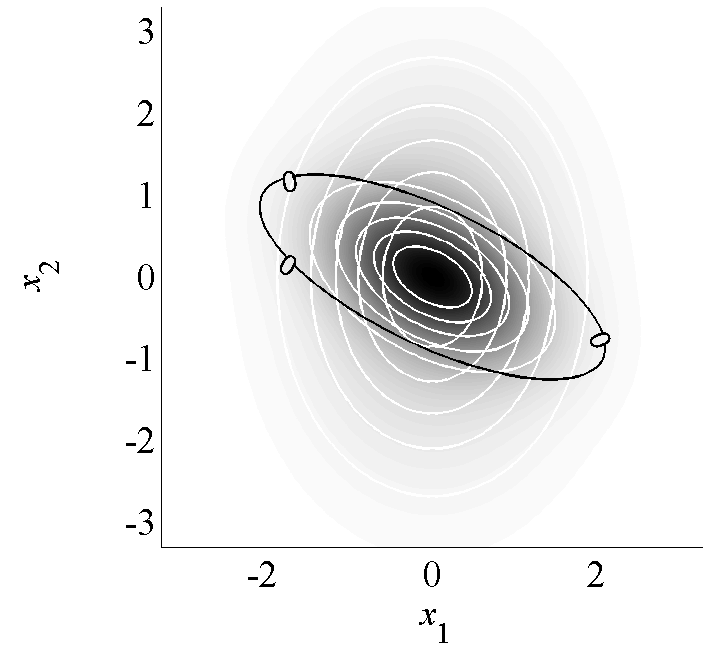
\includegraphics[width=6cm]{Figures/DecGauss2Deqm.pdf}
			\caption{Elliptic decision boundary for a 2D Gaussian problem with zero means.}
			\label{fig:DecGauss2Deqm}
		\end{center}
	\end{figure}
\end{example}

\begin{example}
	Figure \ref{fig:DecGauss2Deqm2} shows the ML decision boundary for 2D Gaussian observations with
	\begin{equation*}
	{\bf m}_0 =  \left(\begin{array}{l}  0\\0   \end{array}\right), {\bf V}_0 = 
	\left(\begin{array}{ll} 0.33 & 0.39 \\ 0.39 & 0.77  \end{array} \right)
	\end{equation*}
	and
	\begin{equation*}
	{\bf m}_1 = \left(\begin{array}{l}  0\\0  \end{array}\right), {\bf V}_1 = 
	\left(\begin{array}{ll} 0.39 &-0.19 \\ -0.19 & 0.16\end{array} \right).
	\end{equation*}
	In this example, the variance under hypothesis $h=1$ is larger only along dimension 1, whereas it is smaller along dimension 2. Hence, as a consequence, the boundary is a hyperbola.
	\begin{figure}[htb]
		\begin{center}
			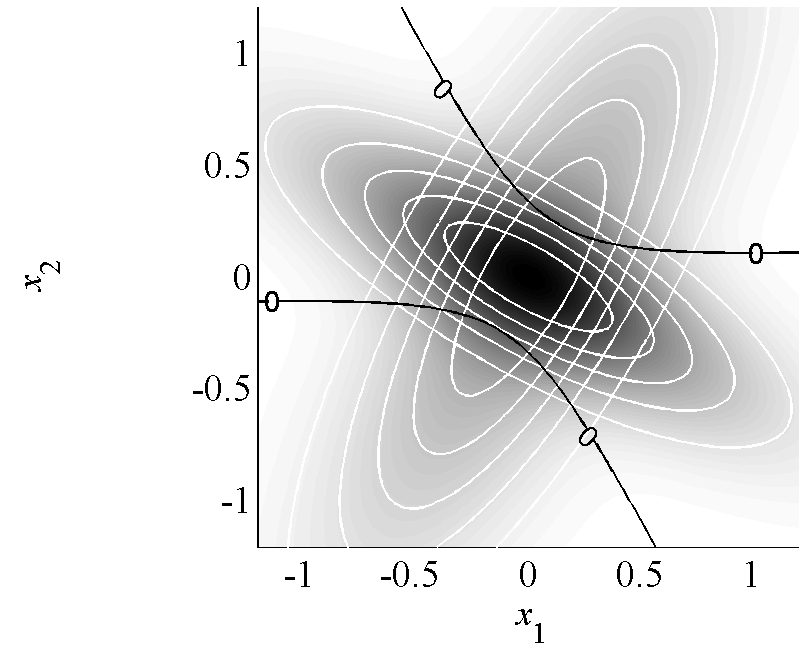
\includegraphics[width=6cm]{Figures/DecGauss2Deqm2.pdf}
			\caption{Hyperbolic decision boundary for a 2D Gaussian problem with zero means.}
			\label{fig:DecGauss2Deqm2}
		\end{center}
	\end{figure}
\end{example}

%\subsection{Summary of most relevant expressions}
%\subsubsection{General case}
%\begin{itemize}
%    \item Probability of error
%    $$P_e = P(D\neq H) = 1 - P(D=H)$$
%    \item Probability of error given ${\bf x}$
%    $$P(d\neq H|{\bf x}) = 1 - P(d = H|{\bf x}) = 1 - P_{H|{\bf X}}(d|{\bf x})$$
%    \item Mean cost
%    $$\mathbb{E}\left\{ c_{DH}\right\} = \sum_{h=0}^{M-1} \sum_{d=0}^{M-1} c_{dh} P(D=d, H=h)$$
%    \item Mean cost given $\bf x$
%    $$\mathbb{E}\left\{ c_{dH}\right|{\bf x}\} = \sum_{h=0}^{M-1} c_{dh} P_{H|X}(h|{\bf x})$$
%    \item ML classifier
%    $$d_{ML} = \arg\max_h p_{{\bf X}|H}({\bf x}|h)$$
%    \item MAP classifier
%    $$d_{MAP} = \arg\max_h P_{H|{\bf X}}(h|{\bf x})$$
%    \item Minimum mean cost classifier
%    $$d^\star = \arg\min_{d} \sum_{h=0}^{M-1} c_{dh} P_{H|X}(h|{\bf x})$$
%\end{itemize}
%
%\subsubsection{Binary case}
%\begin{itemize}
%    \item Probability of error
%    $$P_e = P_\text{M} P_H(1) + P_\text{FA} P_H(0)$$
%    \item Probability of False Alarm, Missing and Detection
%    \begin{align}
%        P_\text{FA} & = P(D=1|H=0) = \int_{{\cal X}_1} p_{\bf X|H}({\bf x}|0) d{\bf x} \nonumber \\
%        P_\text{M} & = P(D=0|H=1) = \int_{{\cal X}_0} p_{\bf X|H}({\bf x}|1) d{\bf x} \nonumber \\
%        P_\text{D} & = P(D=1|H=1) = 1 - P_\text{M} \nonumber
%    \end{align}
%    \item Likelihood ratio test:
%    $$\displaystyle\frac{p_{{\bf X}|H}({\bf x}|1)}{p_{{\bf X}|H}({\bf x}|0)} \dunodcero \eta$$
%    Some particular cases are:
%    \begin{itemize}
%        \item ML classifier: $\eta_{ML} = 1$
%        \item MAP classifier: $\eta_{MAP} = \displaystyle\frac{P_H(0)}{P_H(1)}$
%        \item Minimum mean cost classifier: $\eta^\star = \displaystyle\frac{c_{10}-c_{00}}{c_{01}-c_{11}} \displaystyle\frac{P_H(0)}{P_H(1)}$
%    \end{itemize}
%
%\end{itemize}